% !TeX program = lualatex
% !TeX TXS-program:compile = txs:///lualatex/[--shell-escape]
% Graphs, round three: a legend, a grid, plot marks, a curve clipped to its axes (an
% asymptote), shades of fill hatched to match, and a diagram of nodes and arrows.
% Build:  bin\cacography.cmd graph-demo3
\documentclass{article}
\usepackage[
  paper=notebook,
  ink=blue,
  seed=2718,
  background=oak,
  light=window,
  framing=tight,
  angle=slight,
  crumple=none,
  stains=none,
  props=none,
  backside=none,
]{cacography}
\usepackage{amsmath}
\usepackage{pgfplots}
\usepackage{tikz}
\usetikzlibrary{arrows.meta, positioning}
\pgfplotsset{compat=1.17}

\begin{document}

\section{Two measurements}
\begin{center}
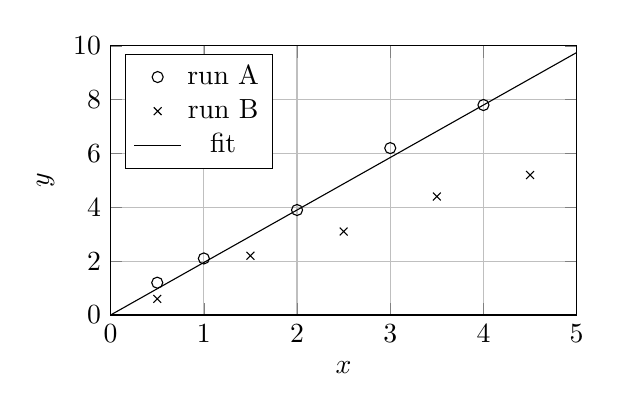
\begin{tikzpicture}
\begin{axis}[width=7.5cm, height=5cm, grid=major, xlabel={$x$}, ylabel={$y$},
             xmin=0, xmax=5, ymin=0, ymax=10, legend pos=north west]
  \addplot[mark=o, only marks] coordinates {(0.5,1.2) (1,2.1) (2,3.9) (3,6.2) (4,7.8)};
  \addlegendentry{run A}
  \addplot[mark=x, only marks] coordinates {(0.5,0.6) (1.5,2.2) (2.5,3.1) (3.5,4.4) (4.5,5.2)};
  \addlegendentry{run B}
  \addplot[domain=0:5, samples=20] {1.95*x};
  \addlegendentry{fit}
\end{axis}
\end{tikzpicture}
\end{center}

\section{A pole at $x=1$}
\begin{center}
\begin{tikzpicture}
\begin{axis}[width=7cm, height=4.6cm, axis lines=middle, xmin=-1, xmax=4, ymin=-6, ymax=6,
             xlabel={$x$}, ylabel={$f$}]
  \addplot[domain=-1:0.9, samples=40] {1/(x-1)};
  \addplot[domain=1.1:4, samples=40] {1/(x-1)};
  \addplot[dashed, domain=-6:6] (1, x);
\end{axis}
\end{tikzpicture}
\end{center}

\section{Shares}
\begin{center}
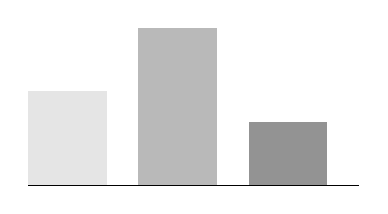
\begin{tikzpicture}
  \fill[gray!20] (0,0) rectangle (1,1.2);
  \fill[gray!55] (1.4,0) rectangle (2.4,2.0);
  \fill[gray!85] (2.8,0) rectangle (3.8,0.8);
  \draw (0,0) -- (4.2,0);
\end{tikzpicture}
\end{center}

\section{The cycle}
\begin{center}
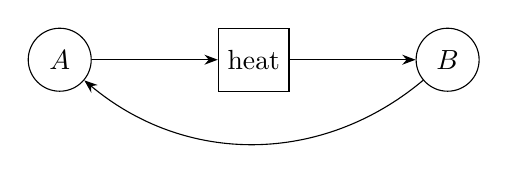
\begin{tikzpicture}[node distance=1.6cm, >=Stealth, every node/.style={draw, minimum size=8mm}]
  \node[circle] (a) {$A$};
  \node[rectangle, right=of a] (b) {heat};
  \node[circle, right=of b] (c) {$B$};
  \draw[->] (a) -- (b);
  \draw[->] (b) -- (c);
  \draw[->] (c) to[bend left=40] (a);
\end{tikzpicture}
\end{center}

\end{document}
